\section{Exercise one}

Consider the process described by the expression: 
\[y(t)=\dfrac{1}{2}y(t-1)+e(t)-e(t-1) \qquad e(t) \sim WN(0,9)\]

\subsection{Solution}
In case of a stationary stochastic process, the following formula holds: 
\[\Gamma_y(\omega)=\left\lvert W(e^{j\omega})\right\rvert^2 \Gamma_u(\omega) = \left\lvert W(e^{j\omega})\right\rvert^2 \lambda^2\]

So, we start by computing the transfer function: 
\[y(t)=\dfrac{z-1}{z-\frac{1}{2}}\]
The pole is inside the unit circle, $e(t)$ is a stationary stochastic process since it is a White Noise. 
Thus, $y(t)$ is a stationary stochastic process, and we can use the fundamental theorem of the spectral analysis: 
\[\Gamma_y(\omega) = \left\lvert \dfrac{e^{j\omega}-1}{e^{j\omega}-\frac{1}{2}}\right\rvert^2 9\]
We compute the squares as: 
\begin{itemize}
    \item $\left\lvert e^{j\omega}-1 \right\rvert^2=\left( e^{j\omega}-1 \right)\left( e^{-j\omega}-1 \right)=2(1-\cos\omega)$
    \item $\left\lvert e^{j\omega}-\frac{1}{2}\right\rvert^2=\left( e^{j\omega}-\frac{1}{2} \right)\left( e^{-j\omega}-\frac{1}{2} \right)=\dfrac{5}{4}-\cos\omega$
\end{itemize}
And so the spectral density function is: 
\[\Gamma_y(\omega) = \dfrac{1-\cos\omega}{\frac{5}{4}-\cos\omega} 18\]
From which we can find the graph: 
\begin{figure}[H]
    \centering
    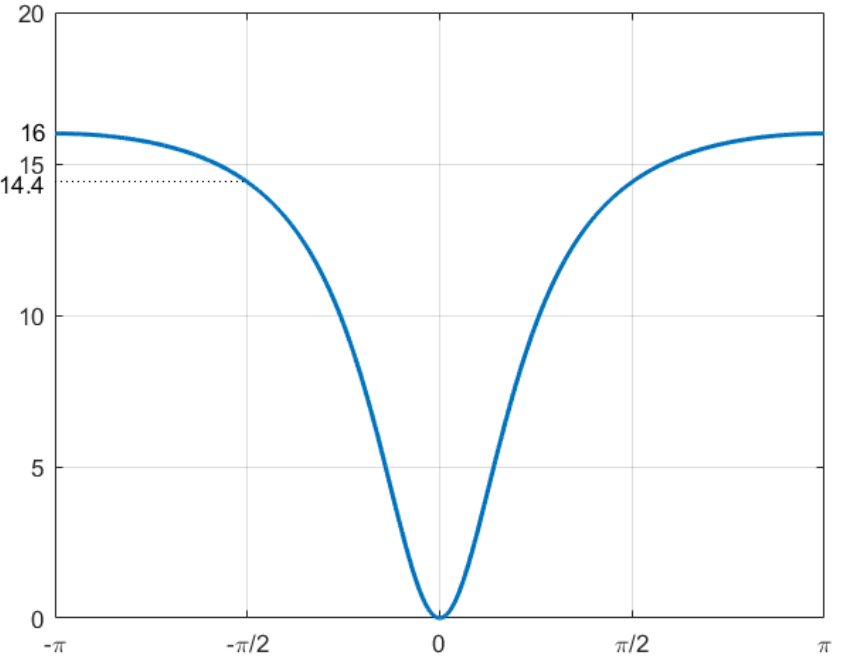
\includegraphics[width=0.5\linewidth]{images/spec.png}
\end{figure}